\documentclass[a4paper,12pt]{article}
\usepackage{tabularx}
\usepackage{amsmath}
\usepackage[utf8]{inputenc}
\usepackage{multicol}
\usepackage{amsmath, amssymb, amsthm}
\usepackage{graphicx}
\usepackage{enumitem}
\usepackage{array}
\usepackage[left=2cm, right=2cm, top=2cm, bottom=2cm]{geometry}
\usepackage{fancyhdr}
\usepackage{xfp}
\usepackage{pgf}
\usepackage{tikz}

\usepackage{graphicx}
\usepackage{fancyhdr}
\setlength{\headheight}{28pt} % genug Platz für das Logo
\pagestyle{fancy}
\fancyhf{} % alles leeren
\fancyhead[L]{\includegraphics[height=1.2cm]{logo.png}}
\fancyhead[C]{\small Klassenarbeit – Funktionale Zusammenhänge\\ Potenzfunktionen \ (Kl. G9A)}
\fancyhead[R]{\small Name:\ \rule{2.8cm}{0.4pt}}
\fancyfoot[C]{\thepage}

\fancyfoot[C]{Seite \thepage \enspace\textbullet\enspace J.\,Mycan \textcopyright~2025}

\renewcommand{\footrulewidth}{0.4pt}




%\pagestyle{fancy}
%\lhead{Klassenarbeit 45min.}
%\chead{Heinrich-von-Kleist-Schule}
%\rhead{Mathematik - G8A}
%\lfoot{}
%\cfoot{Seite \thepage}
%\rfoot{}

\newcommand{\punkteA}{6}
\newcommand{\punkteB}{6}
\newcommand{\punkteC}{6}
\newcommand{\punkteD}{18}
\newcommand{\punkteE}{6}
%\newcommand{\punkteF}{12}

\newcommand{\maxSumme}{42}
\newcommand{\noteEinsMin}{\fpeval{round(\maxSumme * 0.95,0)}}
\newcommand{\noteZweiMin}{\fpeval{round(\maxSumme * 0.80,0)}}
\newcommand{\noteDreiMin}{\fpeval{round(\maxSumme * 0.60,0)}}
\newcommand{\noteVierMin}{\fpeval{round(\maxSumme * 0.45,0)}}
\newcommand{\noteFunfMin}{\fpeval{round(\maxSumme * 0.20,0)}}
\newcommand{\noteSechsMin}{0}

\newcommand{\summe}{%
	\pgfmathparse{\punkteA + \punkteB + \punkteC + \punkteD + \punkteE}%
	\pgfmathprintnumber{\pgfmathresult}}

\begin{document}
	
%	\begin{center}
%		\textbf{Klassenarbeit - Lineare Funktionen und LGS}
%	\end{center}
	
%	\textbf{Vor- und Nachname:} \underline{\hspace{10cm}}\\[0.1cm]
	Die Lösungen sowie Lösungswege sollten klar strukturiert und gut nachvollziehbar sein.\\[0.1cm]
	

	
	
	% -------------------------------------------------
	% Aufgabe 1
	% -------------------------------------------------
	\textbf{Aufgabe 1 ( Punkte)}\\
\textbf{Aufgabe: Zuordnung von Parabeln}\\[0.5em]
Im Koordinatensystem sind vier verschiedene Parabeln eingezeichnet:
zwei nach oben geöffnet, zwei nach unten geöffnet.
Ordne jedem Graphen (I–IV) eine passende Funktionsgleichung zu.
Eine der fünf Funktionsgleichungen passt zu keinem der Graphen.

\begin{center}
	\begin{tikzpicture}[scale=0.9]
		% Koordinatensystem [-5,5] x [-5,5] mit Gitter
		\draw[step=1,very thin,gray!40] (-5,-5) grid (5,5);
		\draw[->] (-5,0) -- (5.5,0) node[below right] {$x$};
		\draw[->] (0,-5) -- (0,5.5) node[above] {$y$};
		
		% Achsenbeschriftung (einige Ticks)
		\foreach \x in {-4,-2,2,4}
		\draw (\x,0.1) -- (\x,-0.1) node[below=2pt] {\small \x};
		\foreach \y in {-4,-2,2,4}
		\draw (0.1,\y) -- (-0.1,\y) node[left=2pt] {\small \y};
		
		% Parabel I: f(x) = 1/4 x^2 - 2  (nach oben geöffnet, Scheitel bei (0|-2))
		\draw[thick,domain=-4.5:4.5,smooth,variable=\x]
		plot ({\x},{0.25*\x*\x - 2});
		\node[below right] at (0,-2) {\small I};
		
		% Parabel II: f(x) = 1/4 (x-2)^2 + 1  (nach oben geöffnet, Scheitel bei (2|1))
		\draw[thick,dashed,domain=-1:5,smooth,variable=\x]
		plot ({\x},{0.25*(\x-2)*(\x-2) + 1});
		\node[above right] at (2,1) {\small II};
		
		% Parabel III: f(x) = -1/4 x^2 + 3  (nach unten geöffnet, Scheitel bei (0|3))
		\draw[thick,dotted,domain=-4:4,smooth,variable=\x]
		plot ({\x},{-0.25*\x*\x + 3});
		\node[above right] at (0,3) {\small III};
		
		% Parabel IV: f(x) = -1/2 (x+3)^2 + 1  (nach unten geöffnet, Scheitel bei (-3|1))
		\draw[thick,loosely dashed,domain=-5:1,smooth,variable=\x]
		plot ({\x},{-0.5*(\x+3)*(\x+3) + 1});
		\node[above left] at (-3,1) {\small IV};
		
	\end{tikzpicture}
\end{center}

\noindent
\textbf{Zuordnungsaufgabe:}\\
Ordne jedem Graphen I–IV genau eine Funktionsgleichung zu.
Eine Funktionsgleichung bleibt übrig.

\begin{itemize}
	\item[A)] \(f(x) = \dfrac{1}{4}x^{2} - 2\)
	\item[B)] \(f(x) = \dfrac{1}{4}(x-2)^{2} + 1\)
	\item[C)] \(f(x) = -\dfrac{1}{4}x^{2} + 3\)
	\item[D)] \(f(x) = -\dfrac{1}{2}(x+3)^{2} + 1\)
	\item[E)] \(f(x) = \dfrac{1}{2}x^{2}\)
\end{itemize}



	
	% -------------------------------------------------
	% Aufgabe 2
	% -------------------------------------------------
	\textbf{Aufgabe 2 ( Punkte)}\\
Die Flugkurve eines Speers entspricht der abgebildeten Parabel und kann durch folgende
quadratische Funktion beschrieben werden:
\[
f(x) = -0,0125 \cdot x^{2} + 0{,}5 \cdot x + 2{,}2.
\]
Dabei werden \(f(x)\) und \(x\) jeweils in Metern gemessen.

\begin{enumerate}
	\item[a)] Ermittle die Abwurfhöhe des Speers.
	\item[b)] Berechne, in welcher horizontalen Entfernung vom Abwurf der Speer gelandet ist.
	\item[c)] Berechne die maximale Flughöhe des Speers.
\end{enumerate}
	
	% -------------------------------------------------
	% Aufgabe 3
	% -------------------------------------------------
	\textbf{Aufgabe 3 ( Punkte)}\\
	Der Zähler eines Bruches ist um 7 größer als dessen Nenner. Werden Zähler und Nenner um
	8 vergrößert, so wird der Bruch um \(\frac{1}{10}\) kleiner als der ursprüngliche Bruch.
	Bestimme alle Brüche, welche diese Eigenschaft erfüllen.\\

%\textbf{Lösung der Gleichung}
%
%Wir haben die Gleichung
%\[
%\frac{x+15}{x+8} = \frac{x+7}{x} - \frac{1}{10}.
%\]
%
%\textbf{1. Schritt: Definitionsbereich}\\
%Im Nenner stehen \(x\) und \(x+8\), also
%\[
%x \neq 0,\quad x \neq -8.
%\]
%
%\textbf{2. Schritt: Brüche durch Multiplikation beseitigen}\\
%Wir multiplizieren beide Seiten mit dem Hauptnenner \(10x(x+8)\):
%\[
%10x(x+8)\cdot \frac{x+15}{x+8}
%=
%10x(x+8)\cdot\left(\frac{x+7}{x} - \frac{1}{10}\right).
%\]
%
%Links kürzt sich \((x+8)\), rechts einmal \(x\) bzw. \(10\):
%\[
%10x(x+15)
%=
%10(x+8)(x+7) - x(x+8).
%\]
%
%\textbf{3. Schritt: Klammern ausmultiplizieren}\\
%Links:
%\[
%10x(x+15) = 10x^2 + 150x.
%\]
%
%Rechts:
%\[
%(x+8)(x+7) = x^2 + 15x + 56,
%\]
%also
%\[
%10(x+8)(x+7) = 10x^2 + 150x + 560,
%\]
%und
%\[
%x(x+8) = x^2 + 8x.
%\]
%
%Damit:
%\[
%10x^2 + 150x
%=
%\bigl(10x^2 + 150x + 560\bigr) - \bigl(x^2 + 8x\bigr)
%=
%9x^2 + 142x + 560.
%\]
%
%\textbf{4. Schritt: Auf eine Seite bringen}\\
%\begin{align*}
%	10x^2 + 150x &= 9x^2 + 142x + 560\\
%	10x^2 - 9x^2 + 150x - 142x - 560 &= 0\\
%	x^2 + 8x - 560 &= 0.
%\end{align*}
%
%\textbf{5. Schritt: Quadratische Gleichung lösen}\\
%Wir faktorisieren:
%\[
%x^2 + 8x - 560 = 0.
%\]
%Gesucht sind zwei Zahlen mit Produkt \(-560\) und Summe \(8\):
%\[
%28 \cdot (-20) = -560,\quad 28 + (-20) = 8.
%\]
%Also
%\[
%x^2 + 8x - 560 = (x+28)(x-20) = 0.
%\]
%
%Damit:
%\[
%x_1 = -28,\quad x_2 = 20.
%\]
%
%Beide Werte sind im Definitionsbereich (\(x\neq 0, -8\)), also zulässig.
%
%\textbf{6. Schritt: Zugehörige Brüche bestimmen}\\
%Der Nenner ist \(x\), der Zähler ist \(x+7\).
%
%\[
%x = -28 \Rightarrow \text{Bruch} = \frac{x+7}{x} = \frac{-28+7}{-28}
%= \frac{-21}{-28} = \frac{21}{28} = \frac{3}{4}.
%\]
%
%\[
%x = 20 \Rightarrow \text{Bruch} = \frac{x+7}{x} = \frac{20+7}{20}
%= \frac{27}{20}.
%\]
%
%\[
%\boxed{\text{Die gesuchten Brüche sind } \frac{3}{4} \text{ und } \frac{27}{20}.}
%\]

	% -------------------------------------------------
	% Aufgabe 4
	% -------------------------------------------------
	\textbf{Aufgabe 4 ( Punkte)}\\
Löse folgende quadratische Gleichungen:
\begin{enumerate}
	\item[a)] \(2x^2 + x - 3 \;=\; x^2 + 5x - 7\)
	
	\item[b)] \((x+2)^2 - 3x \;=\; x^2 - x + 6\)
	
	\item[c)] \(4x^2 - (x-1)^2 \;=\; 2x^2 + 7x - 3\)
\end{enumerate}

	% -------------------------------------------------
	% Aufgabe 5
	% -------------------------------------------------\textbf{Aufgabe: Hängebrücke}\\[0.5em]
	\textbf{Aufgabe 5 ( Punkte)}\\
Die Form des Haupttrageseils der unten abgebildeten Hängebrücke kann in einem
Koordinatensystem näherungsweise durch die quadratische Funktion
\[
h(x) = 0{,}014\,x^{2} + 4
\]
beschrieben werden. Dabei ist \(x\) der waagerechte Abstand von der Brückenmitte
(in Metern) und \(h(x)\) die Höhe des Seils über der Fahrbahn (ebenfalls in Metern).
An den Pylonen \(A\) und \(B\) ist das Seil jeweils \(14\,\text{m}\) über der Fahrbahn
befestigt.

\begin{center}
	\includegraphics[width=\textwidth]{brücke.png}
\end{center}

\noindent
Berechne die \emph{Spannweite} der Brücke, also den horizontalen Abstand der
beiden Befestigungspunkte \(A\) und \(B\) voneinander.

	\newpage
	% -------------------------------------------------
	% Aufgabe 6
	% -------------------------------------------------
	\textbf{Aufgabe 6 ( Punkte)}\\
	Gegeben ist eine quadratische Funktion \(f\). Der Graph von \(f\) besitzt die Nullstellen
	\[
	x_1 = -1 \quad\text{und}\quad x_2 = 3.
	\]
	Außerdem liegt der Punkt
	\[
	P(0\mid -6)
	\]
	auf dem Graphen von \(f\).
	
%\medskip
	Bestimme die Funktionsgleichung von \(f\).\\

	% -------------------------------------------------
	% Aufgabe 7
	% -------------------------------------------------
	\textbf{Aufgabe 7 ( Punkte)}\\
	Ein Feuerwerksflugkörper wird von der Erde aus senkrecht nach oben abgeschossen. 
	Die Flugbahn des Feuerwerkskörpers in einem Koordinatensystem lässt sich näherungsweise 
	durch den Graphen einer quadratischen Funktion beschreiben. 
	
	Dabei gilt:
	\begin{itemize}
		\item Der Abschuss erfolgt im Ursprung des Koordinatensystems, also im Punkt \(A(0\mid 0)\).
		\item Nach \(35\,\text{m}\) horizontaler Entfernung vom Abschuss erreicht der 
		Feuerwerkskörper seine maximale Höhe von \(37\,\text{m}\).
		\item Nach insgesamt \(68\,\text{m}\) horizontaler Entfernung vom Abschuss 
		schlägt der Feuerwerkskörper wieder am Boden auf.
	\end{itemize}
	
	\begin{enumerate}
		\item[] Bestimme den Funktionsterm \(f(x)\), der Funktion die, die Flugbahn des Feuerwerkskörpers beschreibt. \\
	\end{enumerate}
	

	
\end{document}
